% Template for ICASSP-2010 paper; to be used with:
%          mlspconf.sty  - ICASSP/ICIP LaTeX style file adapted for MLSP, and
%          IEEEbib.bst - IEEE bibliography style file.
% --------------------------------------------------------------------------
\documentclass{article}
\usepackage{amsmath,graphicx,mlspconf}

\copyrightnotice{978-1-4673-7454-5/15/\$31.00 {\copyright}2015 IEEE}

\toappear{2015 IEEE International Workshop on Machine Learning for Signal Processing, Sept.\ 17--20, 2015, Boston, USA}


% Example definitions.
% --------------------
\def\x{{\mathbf x}}
\def\L{{\cal L}}

% Title.
% ------
\title{Filtering of Frequency-Transformed Image 
for Privacy Preserving Facial Recognition \\(DRAFT v1.0)}
%
% Single address.
% ---------------
\name{Author(s) Name(s)\thanks{Thanks to XYZ agency for funding.}}
\address{Author Affiliation(s)}
%
% For example:
% ------------
%\address{School\\
%	Department\\
%	Address}
%
% Two addresses (uncomment and modify for two-address case).
% ----------------------------------------------------------
%\twoauthors
%  {A. Author-one, B. Author-two\sthanks{Thanks to XYZ agency for funding.}}
%	{School A-B\\
%	Department A-B\\
%	Address A-B}
%  {C. Author-three, D. Author-four\sthanks{The fourth author performed the work
%	while at ...}}
%	{School C-D\\
%	Department C-D\\
%	Address C-D}
%
\begin{document}
%\ninept
%

\maketitle
%
\begin{abstract}
This paper examines the use of filters on feature vectors for 
privacy protection in facial recognition. Feature vectors are 
the results of Fast Fourier Transform and Wavelet Transform on 
the Yale and Olivetti datasets. Several filters are proposed. 
Filters based on the signal to noise ratio and t test select 
feature which prevent privacy compromising reconstruction without 
sacrificing accuracy. The use of phase removal for FFT and 
normalization are also shown to protect privacy.   
\end{abstract}
%
\begin{keywords}
One, two, three, four, five
\end{keywords}
%
\section{Introduction}
\label{sec:intro}

In modern times, the growth of the Internet and digital sensors has lead to the collection of massive amount of personal information. 
Videos, photos, emails, banking transactions, browsing history, GPS tracks, and other data is collected and store in the cloud  
This data may be circulated around the Internet and severs without the owner's knowledge. The value and scale of the data creates 
the risk of privacy leakage. While encryption has been the traditional solution to this problem, recently a novel privacy preserving 
methodology, compressive privacy, was developed. In the compressive privacy paradigm, the data owner controls the privacy of the data 
before uploading it to the cloud [need to cite Prof Kung].    
\\\\
As noted in \cite{bowyer2004face}, 9/11, Edward Snowden incident and other events have resulted in both a demand for 
recognition systems and a concern for privacy violation by such systems. A critical competent of such system is biometric identification of people, 
mainly by facial recognition which can be performed in without consent and at a distnce by suvellance camreas. 
While a lot of research has gone into improving facial recognition systems - \cite{bouzalmat2014comparative}, 
\cite{spies2000face}, \cite{bouzalmat2011facial}, 
\cite{dehai2013pca}, \cite{samra2003face} among others - relatively little research has been done on incorporating privacy into such systems; 
some examples being \cite{erkin2009privacy}, \cite{sadeghi2010efficient}, and \cite{kevenaar2005face}.    
\\\\
The primary approach to privacy in facial recognition is cryptography. In \cite{erkin2009privacy}, 
Eigenfaces recogition system is used on homomorphically encrypted data. In this first cryptographic system 
for facial recognition \cite{erkin2009privacy}, the client wants the server to identify a face without revealing 
the image to the server. The server also does not want to reveal the contents of it's database. In this approach, 
data is quantized for Pailler encryption and server and client share computations needed for matching faces.
\cite{erkin2009privacy} Experimentally, 96\% accuracy was achieved in \cite{erkin2009privacy} on "ORL Database of Faces". 
\cite{sadeghi2010efficient} improved the algorithm presented in \cite{erkin2009privacy} by reducing the time and space 
complexity with the use of garbled circuits. 
\\\\
Along a different line of research, \cite{kevenaar2005face} used Helper Data Systems to provide privacy. The approach generates binary 
feature vector by determining reliable bits based on statistics from sample data. While the proposed process is similar to compressive
privacy, it leaves pirvacy up to the cloud server and [......................................................................] 
\\\\
Our compressive privacy appoach to facial recognition rests on the idea that privacy is compromised when an image can be visually 
inspected by an unautorized individual. Therefore, as long as the reconstruction of an image from a feature vector is not meaningful 
to a human, privacy has been maintained. Facial recognition systems often utilize Fast Fourier Transform (FFT) or Wavelet Transform (WT) 
as part of feature engineering. For example \cite{spies2000face}, \cite{bouzalmat2011facial}, 
\cite{dehai2013pca}, and \cite{samra2003face} use FFT or WT. In recognition systems like these, it is possible to 
alter the output of FFT or WT to reduce the quality of the reconstructed image without sacrificing accuracy of the classification.           

\section{Our Classification Systems}
\label{sec:system}

We can break down a facial recognition system into two compnents, feature engineering and
classification. Both compenents can be made up of several parts, for example several sequecnail WT transforms. 
We limit our feature engineering to one transform to keep image reconstruction simple, however this may be 
a real constraint in time or power sensative applications. 
As pictured in Figure \ref{fig:mysys}, our classification systems for this investigation, 
begin with an application of FFT or WT to an image. 
Then a filter is applied as part of feature selection. Classification is 
accomplished with an SVM. For all of the following experiments an SVM with a 
leaner kernel and C = 1 was found to produce the best results.    

\begin{figure}[htb]

\begin{minipage}[b]{1.0\linewidth}
  \centering
  \centerline{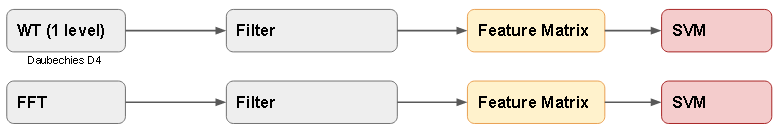
\includegraphics[width=8.5cm]{mysys}}
%  \vspace{2.0cm}
\end{minipage}
%
\caption{Block diagrams of classification systems used.}
\label{fig:mysys}
%
\end{figure}

\section{Filters}
\label{sec:Filters}

Part of our compressive privacy results from the use of filters for feature selection of 
FFT and WT frequencies. A filter is a binary matrix which selects features based on some 
selecting function. 
Let $F_{x,d}$ be a filter $F_{x,d} \in \{0,1\}^{d x m}$ where $m$ is the number of features in each example, $x$ is one of the selecting functions, and $d$ is the number of features selected by the filter.
\\\\
$F_{x, d,i,j} = 1$ if $W_{x}(j)$ is with in the $d$ largest $W_{x}$, otherwise $F_{d,i,j} = 0$. Thus $m$ dimensional feature vectors are compressed to $d$ dimension feauter vectors, based on the ordering of $W_{x}$.
\\\\
Let $X$ be feature vectors for an example: 

\begin{equation} \label{compress}
X_{filtered} =  F_{x,d}X
\end{equation}

$\\$
Selection functions assign a weight to each feature and divide filters into three categories: 
data independent, unsupervised, and supervised. Data indepednent filters do not utalize a traning set 
when determining which features should be selected. In our investigation the Rectangle and Triangle filters 
are data indepednet as they select a predefined region of features. The variance based filter is unsuperived in the 
sense that it does not consider labels of the training examples. Feature selection is done purely based on the 
variance of each feature accross the training set. The idea for this filter originates in \cite{spies2000face}.
\\\\
We devised four supervised filters based on the signal to noise ratio, 
Fisher discriminant ratio, symmetric divergence and t statistical tests. The supervised filters require labels for positive and negative classes. 
During training, for each individual the training examples are divided into two classes. Positive class contains the pictures of that 
individual and the negative class contains all other pictures. The signal to noise ratio, Fisher discriminant ratio, 
symmetric divergence and t tests are computed based on those two classes for each feature, and the final weight for a 
feature is the mean of weights cross all of the individual in the training set.
\\\\
The filters are mathematically defined below. For the equations below, let $\mu^{+}_{j}$, $\sigma^{+}_{j}$, and $N^{+}_{j}$ be 
the mean, standard deviation and number of examples for a target individual and let $\mu^{-}_{j}$, $\sigma^{-}_{j}$, and 
$N^{-}_{j}$ be the mean, standard deviation and number of examples for all other people in the training set. Let $\bar{X}$ be 
the mean of $X$ with respect to the training set in the case of unsurprised filters,
and with respect to all individuals.   

\subsection{Variance}

\begin{equation} \label{Var}
W_{VAR}(j) = \sigma^{2}_{j}
\end{equation}

\subsection{Signal to Noise Ration}

\begin{equation} \label{SNR}
W_{SNR}(j) = \overline{\dfrac{| \mu^{+}_{j} - \mu^{-}_{j} |}{\sigma^{+}_{j} + \sigma^{-}_{j}}}
\end{equation}

\subsection{Fisher Discriminant Ratio}

\begin{equation} \label{FDR}
W_{FDR}(j) = \overline{\dfrac{( \mu^{+}_{j} - \mu^{-}_{j} )^{2}}{(\sigma^{+}_{j})^{2} + (\sigma^{-}_{j})^{2}}}
\end{equation}

\subsection{Symmetric Divergence}

\begin{equation} \label{SD}
W_{SD}(j) = \overline{\dfrac{1}{2} \dfrac{(\mu^{+}_{j})^{2}}{(\mu^{-}_{j})^{2}} + \dfrac{(\mu^{-}_{j})^{2}}{(\mu^{+}_{j})^{2}} + \dfrac{1}{2} \dfrac{( \mu^{+}_{j} - \mu^{-}_{j} )^{2}}{(\sigma^{+}_{j})^{2} + (\sigma^{-}_{j})^{2}} - 1}
\end{equation}

\subsection{T}

\begin{equation} \label{T}
W_{T}(j) = \overline{\dfrac{ \mu^{+}_{j} - \mu^{-}_{j}}{\sqrt{\dfrac{(\sigma^{+}_{j})^{2}}{N^{+}_{j}} + \dfrac{(\sigma^{-}_{j})^{2}}{N^{-}_{j}}}}}
\end{equation}

\subsection{Rectangle}

let $J$ be a rectangular region of features \\

\begin{equation}
W_{Rect}(j) = 
\begin{cases}
	1 & \text{if } j \in J \\
	0 & \text{otherwise}
\end{cases}
\end{equation}

\begin{figure}[htb]

\begin{minipage}[b]{1.0\linewidth}
  \centering
  \centerline{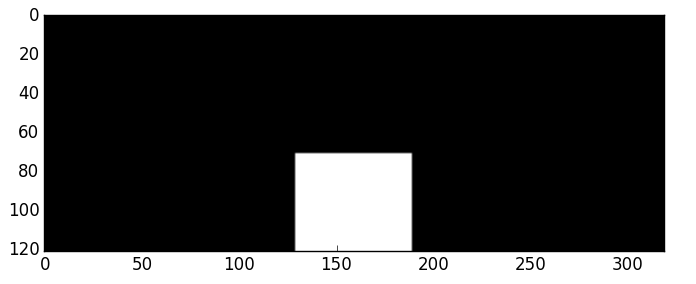
\includegraphics[width=8.5cm]{rect}}
%  \vspace{2.0cm}
\end{minipage}
%
\caption{White pixels represent selected features. The region is indented to select amplitudes of low frequencies in the FFT transform. }
\label{fig:res}
%
\end{figure}

\subsection{Triangle}

Along with the Rectangle filter, this filter was inspired by results in \cite{spies2000face}, 
where features with high varince after FFT are the amplitues of low frequencies and 
they form a trianglar region. 
\\\\
let $J$ be a triangular region of features \\

\begin{equation}
W_{Tri}(j) = 
\begin{cases}
1 & \text{if } j \in J \\
0 & \text{otherwise}
\end{cases}
\end{equation}

\begin{figure}[htb]

\begin{minipage}[b]{1.0\linewidth}
  \centering
  \centerline{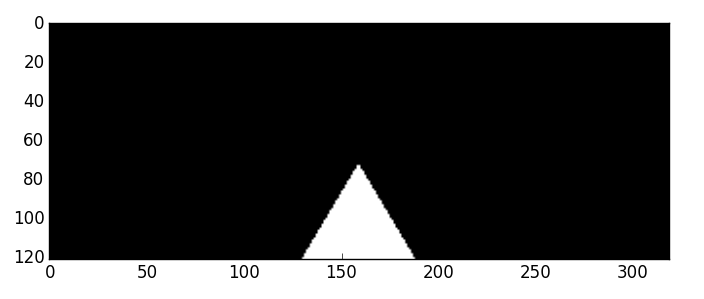
\includegraphics[width=8.5cm]{tri}}
%  \vspace{2.0cm}
\end{minipage}
%
\caption{White pixels represent selected features. The region is indented to select amplitudes of low frequencies in the FFT transform.}
\label{fig:res}
%
\end{figure}

\section{Methods}
\label{sec:Method}

\subsection{Classification}

Ten fold cross validation was used to test classification accuracies. Grid Search was used to optimize the SVM parameters 
for each fold. For all of the following experiments an SVM with a leaner kernel and C = 1 was found to produce the best results. 
100 cross validations were performed and the training of supervised and unsupervised filters was constrained to the appropriate fold. 
Since the rectangle and triangle filters are parameterized by a region they were used to determine $d$ for all other filters. For FFT, the filters 
where only applied to the amplitudes of frequencies. For WT, the filters were applied to all four [....................................].     

\subsection{Reconstruction}

To reconstruct original images from filtered feature vectors, we set the values of all filtered features which were filtered out to be zero.
The operation can be viewed as muliplication by the transpose of the filter.  

\begin{equation}
\tilde{X} =  F_{x,d}^{T}X_{filtered}
\end{equation}

Then the inverse of the FFT or WT is applied on $\tilde{X}$. As mentioned above, only one transform was used at a time to keep this process simple. 


\section{Experimental Results}
\label{sec:ExperimentalResults}

Our baseline accuracy with the FFT transform is 0.741 for the Yale database and 0.975 for the Olivetti database.   
With the WT transform, our baseline for Yale database is 0.807 and for the Olivetti database is 0.963.

\subsection{Phase Removal}

FFT produces amplitudes and phases for transformed image. 
If the phase is removed and the image is reconstructed based on the amplitude the 
result is a faceless image as seen in Figure \ref{fig:nophase}. This clearly protects 
privacy. The cost in accuracy is small. The accuracy drops 0.006 to 0.735 for the Yale database
and by 0.001 to 0.974 for Olivetti database. 

\begin{figure}[!htb]
\begin{minipage}[b]{.48\linewidth}
  \centering
  \centerline{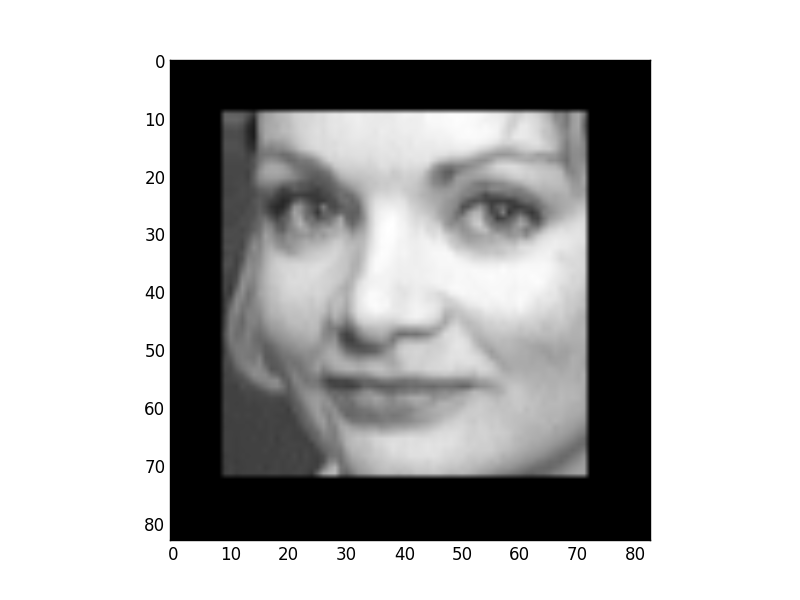
\includegraphics[width=4.0cm]{recon/Original1o}}
%  \vspace{1.5cm}
  \centerline{Original Image}\medskip
\end{minipage}
\hfill
\begin{minipage}[b]{0.48\linewidth}
  \centering
  \centerline{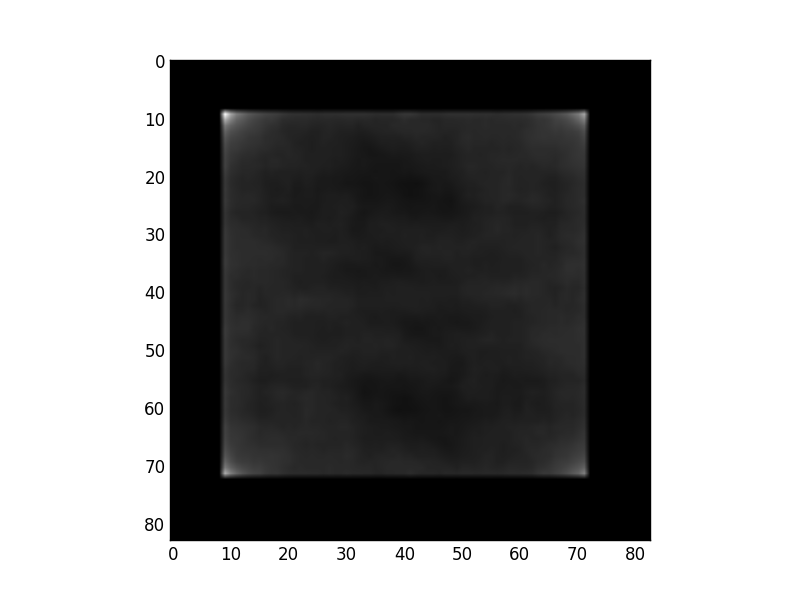
\includegraphics[width=4.0cm]{recon/Recon1o}}
%  \vspace{1.5cm}
  \centerline{Reconstruction}\medskip
\end{minipage}
%
\caption{Result of reconstruction of a FFT transformed image with the phase removed.}
\label{fig:nophase}
%
\end{figure}


\subsection{Normalization}

The amplitudes and phases of the FFT results for the training set can 
be normliazed. Normalization is done by computing the mean and standard 
deviation for each feature and then from each corresponding feature subtracting the mean 
and dividng the difference by the standard deviation. Performing reconstruction 
on the amplitudes and phases without undoing the transformation produces privacy as seen 
in Figure \ref{fig:norm}. On the Olliveti database the accuracy was 0.975. On the Yale database the accuracy was 0.739.

\begin{figure}[!htb]

\begin{minipage}[b]{.48\linewidth}
  \centering
  \centerline{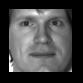
\includegraphics[width=4.0cm]{recon/denorm_Yale}}
%  \vspace{1.5cm}
  \centerline{Original Image}\medskip
\end{minipage}
\hfill
\begin{minipage}[b]{0.48\linewidth}
  \centering
  \centerline{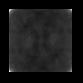
\includegraphics[width=4.0cm]{recon/norm_Yale}}
%  \vspace{1.5cm}
  \centerline{Reconstructed Image}\medskip
\end{minipage}
%
\caption{Reconstruction from normalized FFT output.}
\label{fig:norm}
%
\end{figure}

\subsection{Filtering}

\subsubsection{FFT}

Based on accuarcies in Figure \ref{fig:accFFT}, the T filter has the best or near best 
accuarcy across both datasets. Figure \ref{fig:reconFFT} shows that it also preserves privacy. 
Comapored to the other filters, the face is brealy visible in the reconstrcution from feaures selcted 
by the T filter. 

\begin{figure}[!htb]

\begin{minipage}[b]{1.0\linewidth}
  \centering
    \begin{tabular}{ | l || c | c |}
    \hline
    Filter & Yale Acc & Olliveti Acc \\ \hline
    Rect & 0.737 & 0.967 \\ \hline
    Var & 0.739 & \textbf{0.970} \\ \hline 
    SNR & 0.739 & 0.968 \\ \hline
    FDR & 0.735 & 0.965 \\ \hline
    SD & 0.686 & 0.952 \\ \hline
    T & \textbf{0.741} & 0.968 \\
    \hline
    \end{tabular}
\end{minipage}
%
\caption{Mean accuracy for the filters based on 100, 10 fold cross validations. Top 399 features are
selected.}
\label{fig:accFFT}
%
\end{figure}

\begin{figure} [!htb]

\begin{minipage}[b]{.48\linewidth}
  \centering
  \centerline{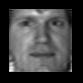
\includegraphics[width=4.0cm]{recon/rectF_399_yale}}
%  \vspace{1.5cm}
  \centerline{Rect 0.73}\medskip
\end{minipage}
\hfill
\begin{minipage}[b]{0.48\linewidth}
  \centering
  \centerline{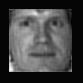
\includegraphics[width=4.0cm]{recon/varF_399_yale}}
%  \vspace{1.5cm}
  \centerline{Var 0.739}\medskip
\end{minipage}
%
\begin{minipage}[b]{.48\linewidth}
  \centering
  \centerline{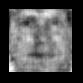
\includegraphics[width=4.0cm]{recon/snrF_399_yale}}
%  \vspace{1.5cm}
  \centerline{SNR 0.739}\medskip
\end{minipage}
\hfill
\begin{minipage}[b]{0.48\linewidth}
  \centering
  \centerline{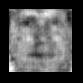
\includegraphics[width=4.0cm]{recon/tF_399_yale}}
%  \vspace{1.5cm}
  \centerline{T 0.741}\medskip
\end{minipage}
%
\caption{Reconstructed images after a FFT transform and filter $d = 399$. The filter name and accuracy on the 
Yale dataset is listed under each image.}
\label{fig:reconFFT}
%
\end{figure}

\subsubsection{WT}

Using the result of the wavelet transform, the T filter still produces 
best or second best accuracires across the two datasets. 

\begin{figure}[!h]

\begin{minipage}[b]{1.0\linewidth}
  \centering
    \begin{tabular}{ | l || c | c |}
    \hline
    Filter & Yale Acc & Olliveti Acc \\ \hline
    Var & 0.737 & 0.941 \\ \hline 
    SNR & \textbf{0.813} & 0.968 \\ \hline
    FDR & 0.807 & \textbf{0.969} \\ \hline
    SD & 0.672 & 0.883 \\ \hline
    T & 0.812 & \textbf{0.969} \\
    \hline
    \end{tabular}
\end{minipage}
%
\caption{Mean accuracy for the filters based on 100, 10 fold cross validations. Top 399 features are
selected.}
\label{fig:res}
%
\end{figure}

As seen in Figure \ref{fig:wtRecon}, the T filter preserves provcary. The reconstructions
for Var and T are similar to reconstrcutiosn for the other filters. The privacy protections 
appears to be a property of the WT tranform rather than any particlar filter. 

\begin{figure}[!htb]

\begin{minipage}[b]{.48\linewidth}
  \centering
  \centerline{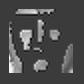
\includegraphics[width=4.0cm]{recon/varF_399_yaleWL}}
%  \vspace{1.5cm}
  \centerline{Var 0.737}\medskip
\end{minipage}
\hfill
\begin{minipage}[b]{0.48\linewidth}
  \centering
  \centerline{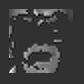
\includegraphics[width=4.0cm]{recon/tF_399_yaleWL}}
%  \vspace{1.5cm}
  \centerline{T 0.812}\medskip
\end{minipage}
%
\caption{Reconstructed images after a WT transform and filter $d = 399$. The filter name and accuracy on the 
Yale dataset is listed under each image.}
\label{fig:wtRecon}
%
\end{figure}


% To start a new column (but not a new page) and help balance the last-page
% column length use \vfill\pagebreak.
% -------------------------------------------------------------------------
\vfill
\pagebreak

\section{Discussion}
\label{sec:conclusion}

$\\$
There is a lot of potential for privacy protection with proper alterations in the feature engineering process. 
Across all of the methods, the cost, in the form of accuracy loss, is very small. In fact, for the wavelett transform, 
the accuracy increased when filters where applied. Additionally, the reconstructions from wavelett transform features 
yieled much better privacy by completely remoeving the eyes and mouth in the image. It appears that the wavelett transform
forms a very good basis for privacy preserving feature vectors. 
\\\\

\begin{figure}[!h]

\begin{minipage}[b]{1.0\linewidth}
  \centering
    \begin{tabular}{ | l | c | c |}
    \hline
    Mathod & From Yale & From Olliveti \\ \hline
    Phase Removal & -0.006 & -0.001 \\ \hline 
    Normalization & -0.002 & 0.000 \\ \hline
    Filtering (FFT) & 0.000 & -0.006 \\ \hline
    Filtering (WT) & 0.005 & 0.006 \\ \hline
    \end{tabular}
\end{minipage}
%
\caption{Changes in mean accuracy relative to the baseline for the four different methods. The T filter is used
for filtering accuracies.}
\label{fig:res}
%
\end{figure}



$\\$
While FFT based systems lost accuracy under all of these methods, it is easier to 
see why the filters preserve accuarcy. The supervised statistical filters select both high and low fequecies 
as seen in Figure \ref{fig:spec}. Therefore, the reconstrcution is not just a blurried image as 
is the case with selecting just the low frequcies. Fewer of those frequcies are selected thus the image 
is even more blurred, but accuarcy is preserved by the high frequeices. The mix avoid details form being reconstructed fully. 

\begin{figure}[!htb]

\begin{minipage}[b]{.48\linewidth}
  \centering
  \centerline{
\includegraphics[width=4.0cm]{filter/rectF_399}}
%  \vspace{1.5cm}
  \centerline{Rect}\medskip
\end{minipage}
\hfill
\begin{minipage}[b]{0.48\linewidth}
  \centering
  \centerline{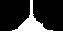
\includegraphics[width=4.0cm]{filter/varF_399}}
%  \vspace{1.5cm}
  \centerline{Var}\medskip
\end{minipage}
%
\begin{minipage}[b]{.48\linewidth}
  \centering
  \centerline{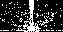
\includegraphics[width=4.0cm]{filter/snrF_399}}
%  \vspace{1.5cm}
  \centerline{SNR}\medskip
\end{minipage}
\hfill
\begin{minipage}[b]{0.48\linewidth}
  \centering
  \centerline{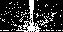
\includegraphics[width=4.0cm]{filter/tF_399}}
%  \vspace{1.5cm}
  \centerline{T}\medskip
\end{minipage}
%
\caption{Amplituedes selected by the filter (marked in white).}
\label{fig:spec}
%
\end{figure}


Regarding the filters, which should be applied even for performance improvements, 
SNR and T are the most useful for privacy protection. For both FFT and WT, these filters allow a 
large dimension reduction with almost no accuracy loss.  
\\\\
In future research consecutive search methods can be utilized to produce filters. Additionally, the reconstruction 
for WT should be explained in terms of the underlying bands. Lastly, a fully algorithm utilizing the filters and taking 
into the account the client server model should be developed.  
\\\\\\\\
This paper represents my own work in accordance with University regulations.              
\\\\\\\\

% References should be produced using the bibtex program from suitable
% BiBTeX files (here: strings, refs, manuals). The IEEEbib.bst bibliography
% style file from IEEE produces unsorted bibliography list.
% -------------------------------------------------------------------------
\bibliographystyle{IEEEbib}
\bibliography{sources} 

\end{document}
